\section{Task 1} \label{ex_1}

\subsection{Time Domain - RMS}

\textbf{RMS} (Root Mean Square Energy) é um descritor temporal que é usado para caracterizar um som, nomeadamente através da sua energia em cada frame.
Tal como o nome indica, é RMS é a raiz quadrada da média da energia do sinal numa determinada janela temporal. 

O RMS é um bom indicador da vitalidade do som num determinado momento. Quanto maior for a janela temporal, menos suscetível será o RMS a mudanças no som.
Temos portanto um trade-off na análise temporal do som. \cite{rms}.

Esperamos que quanto mais intenso for um som, maior será o RMS. À medida que o som diminui de intensidade, o RMS vai diminuir gradualmente.
Para avaliar este descritor temporal, foram escolhidos dois sinais, WGN e uma onda sinusoidal.

Com uma janela temporal média, esperamos que no caso do WGN, o RMS seja relativamente pequeno e irregular, dado que a amplitude do sinal é baixa e insconstante.
Para o caso da onda sinusoidal, o valor médio é bastante mais alto e o sinal periódico.

\begin{figure}[H]
    \centering
    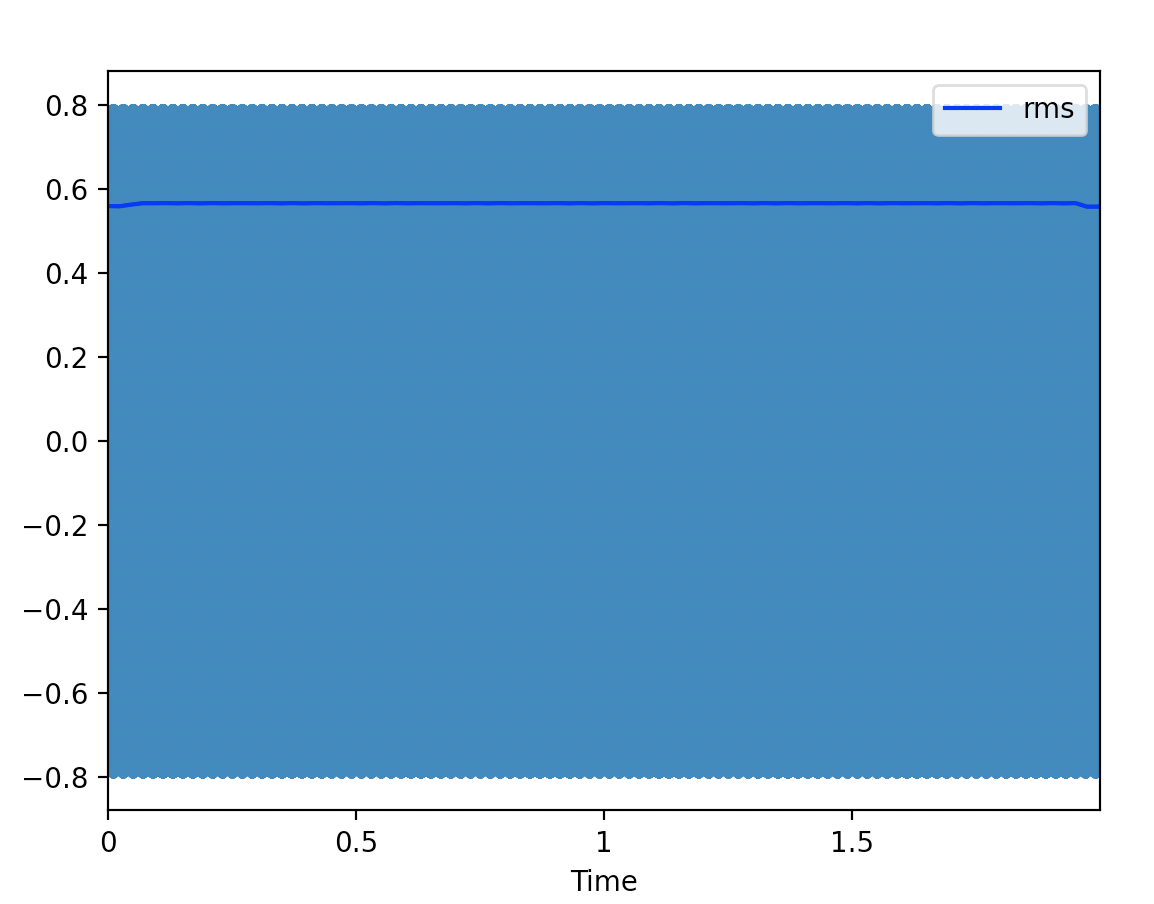
\includegraphics[width=.8\linewidth]{figs/image_1.png}
    \caption{RMS de uma onda sinusoidal}
    \label{fig:rms_1}
\end{figure}

\begin{figure}[H]
    \centering
    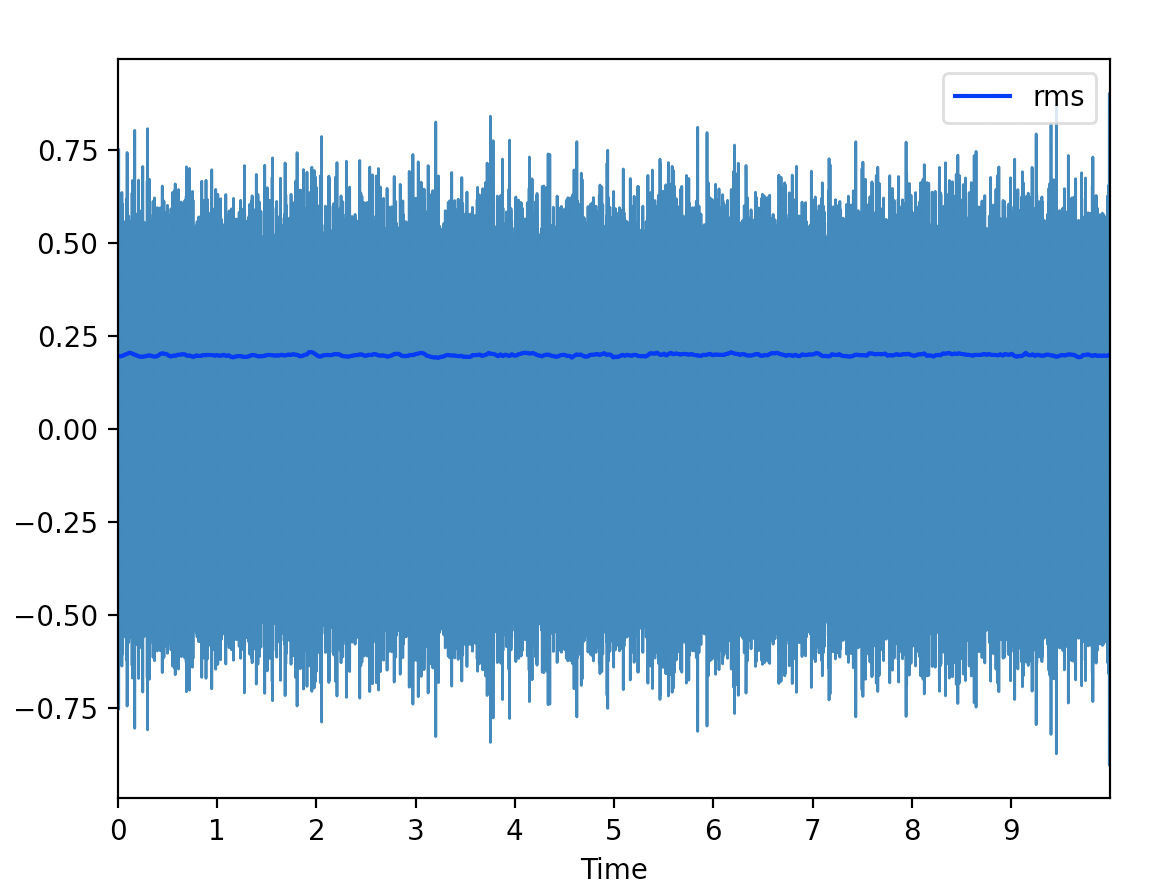
\includegraphics[width=.8\linewidth]{figs/image_2.png}
    \caption{RMS de WGN}
    \label{fig:rms_2}
\end{figure}

Como se pode avaliar pelos resultados obtidos, no caso da onda sinusoidal o RMS é constante após um curto período de tempo para estabilizar (janela temporal ser preenchida).
No caso do WGN, percebemos que o valor não é constante, apresentando várias flutuações ao longo do tempo. O seu valor médio é também mais pequeno.
Note-se que é possível obter um valor de RMS mais estável no caso da WGN se aumentarmos a janela temporal durante o seu cálculo.



\subsection{Frequency Domain - Spectral Spread}
O \textbf{Spectral Spread} é definido como o espalhamento do espectro de uma sinal em torno do seu valor médio.
Assim , é expectável que sons semelhantes a ruído , que possuem um espectro mais largo, tenham um espalhamento espectral maior quando comparados com um som com uma banda mais estreita, dito "tonal". \cite{spec_features}

Para demonstrar isto , calculamos o espectro dos dois sinais seguintes. A figura \ref{fig:ss_1} representa um exemplo de ruído branco e a figura \ref{fig:ss_2} representa uma onda sinusoidal a 1000Hz.
\begin{figure}[H]
    \centering
    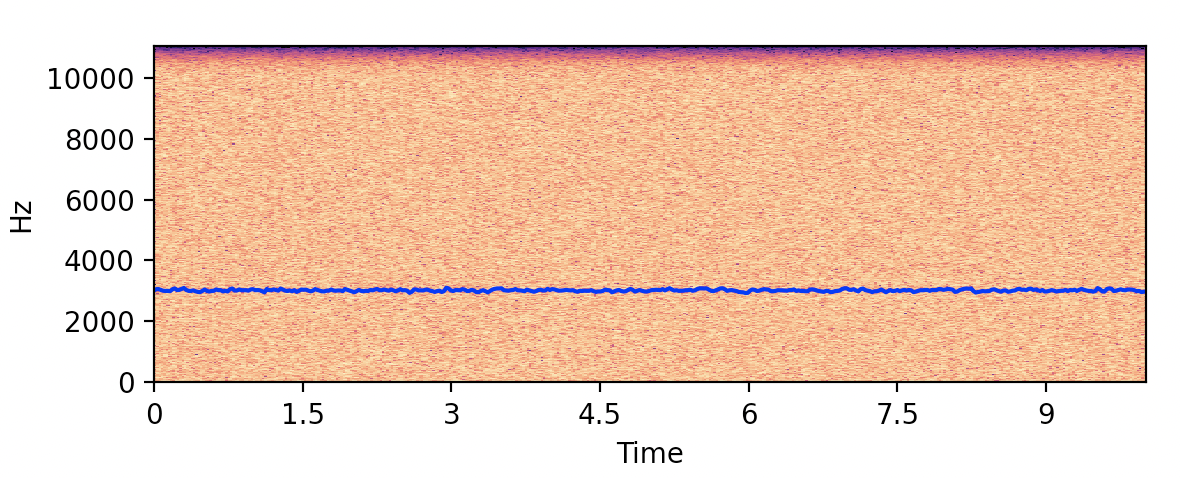
\includegraphics[width=.8\linewidth]{figs/image_3.png}
    \caption{Spectral Spread de WGN}
    \label{fig:ss_1}
\end{figure}

\begin{figure}[H]
    \centering
    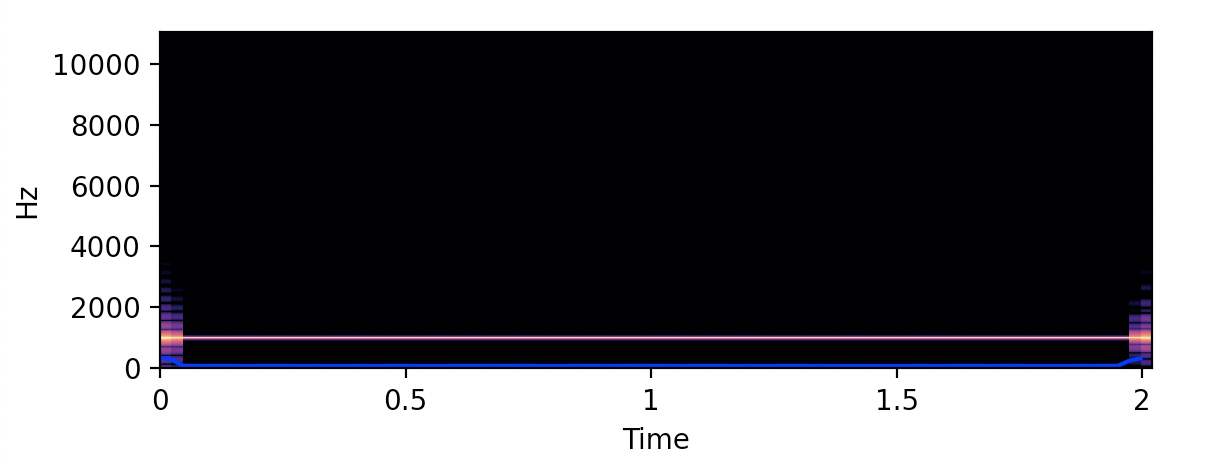
\includegraphics[width=.8\linewidth]{figs/image_4.png}
    \caption{Spectral Spread de uma onda sinusoidal}
    \label{fig:ss_2}
\end{figure}

Obtivemos os valores de espalhamento espetral para o ruído branco de 3020.96 e para a onda sinusoidal de 93.094.
Ou seja, tal como esperado , o valor médio do ruído branco é bastante superior ao da onda sinusoidal.


\section{Task 2} \label{ex_2}

Para esta tarefa , decidimos escolher 1 instrumento de cada tipo (corda , sopro e percussivo) e calcular os descritores instantâneos.
A representar os instrumentos de sopro ,escolhemos a flauta (flt\_G4\_12), para as cordas , o violoncelo (vcl\_a\_G3) e
Não se apresenta resultados para um som percussivo pois não foi fornecido nenhuma sample.

\begin{figure}[H]
    \centering
    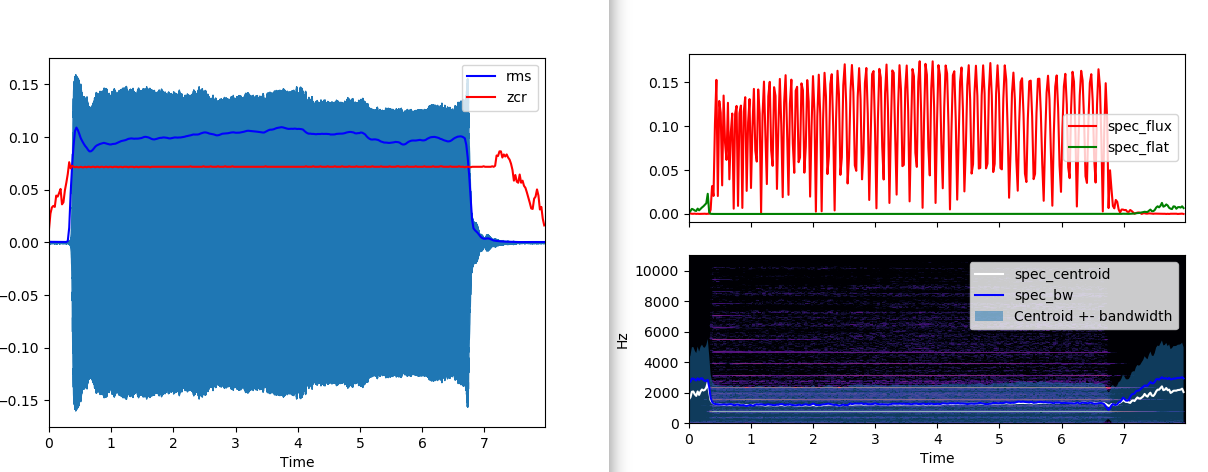
\includegraphics[width=.8\linewidth]{figs/flt_G4_12.png}
    \caption{Instrumento de cordas}
    \label{fig:task2_1}
\end{figure}

\begin{figure}[H]
    \centering
    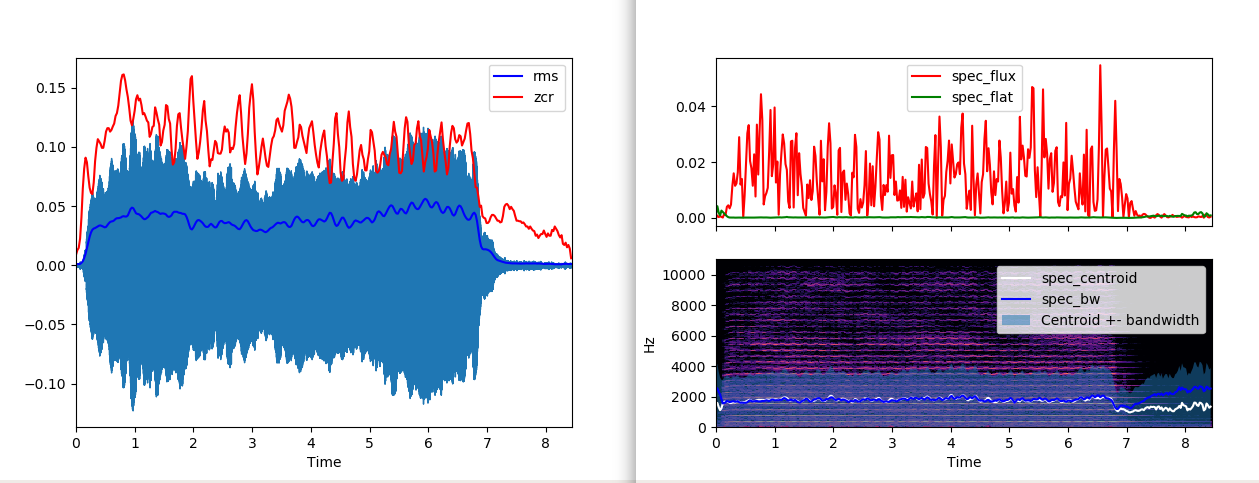
\includegraphics[width=.8\linewidth]{figs/vcl_a_G3_12.png}
    \caption{Instrumento de sopro}
    \label{fig:task2_2}
\end{figure}


O descritor \textbf{RMS} é diferente nos dois instrumentos sendo mais constante no instrumento de cordas.
Isto deve-se ao tipo de excitação dos instrumentos de sopro, onde a vibração labial do executante é mais inconstante do que o arco do violoncelo.

No caso do \textbf{Zero Crossing Rate}, este indica quantas vezes o sinal passa o eixo x ou "0".
Este então relacionado com a frequência da nota que se está a tocar.
Como os dois instrumentos estão a tocar em oitavas diferentes, este parâmetro também vai ser diferente. \cite{zcr}

\textbf{Spectral Flatness} ou "coeficiente de tonalidade" consegue dizer-nos o quão próximo de um "tom" um som é , em oposição a ser parecido 
com ruído branco. Podemos constatar que nos nossos gráficos,tanto no caso do violoncelo como no da flauta, a "spectral flatness" é representada por um valor constantemente muito baixo e próximo de zero.
Isto diz-nos que o espectro de potência do som produzido por estes dois instrumentos está concentrado numa banda de frequências muito pequena. \cite{spec_features}

O \textbf{Spectral Flux} mostra o quão rapidamente o espectro de potência de um som está a mudar e é normalmente usado para determinar o timbre de um som.
O gráfico mostra-nos que os valores do fluxo espectral da flauta (entre 0.05 a 0.15) são bastante superiores aos do violoncelo(entre 0.02 e 0.04).
Este tem um valor mais elevado no caso do instrumento de sopro mas o instrumento de corda tem um gráfico muito mais estável. \cite{spec_features}

Em relação ao \textbf{Spectral Centroid}, este representa onde se localiza o "centro de massa" do espectro do som capaz de realçar as diferenças de frequência do som.
Este é um indicador similar ao Zero Crossing Rate mas no domínio das frequência. \cite{spec_features}.

Por fim, temos o \textbf{Spectral Spread}. Como estamos na presença de sons tonais, ambos os valores são pequenos, não sendo um bom indicador de distinção entre estes sons. \cite{spec_features}

\section{Task 3} \label{ex_3}

\subsection{Descritores Globais}

Após a implementação de funções capazes de obter estes parâmetros num script \textit{Python}, foi feita uma análise estatística destes com o intuito de os utilizar para comparar as diferentes samples de som.
Para cada samples de som , foi calculado:
\begin{itemize}
    \item Spectral Flux médio
    \item Spectral Spread médio
    \item Spectral Flatness médio
    \item Spectral Centroid médio
    \item Zero Crossing Rate médio
    \item Temporal Centroid normalizado
    \item Log Attack Time normalizado
\end{itemize}

O \textbf{Temporal Centroid} e \textbf{Log Attack Time} foram normalizados para que se possa comparar samples de diferentes durações.
Isto deve-se ao facto de os seus valores serem influenciados pela duração da sample pois são apresentados em segundos.

Os resultados foram compilados numa spreadsheet para se proceder a uma futura análise.

\textbf{Log Attack Time} é um logaritmo, que significa que quanto maior for o seu valor negativo, menor é o attack-time.
Este descritor indica o tempo para o som atingir o 90\% do seu valor máximo. É um valor que é representado quando se elabora o \textit{envelope} de um som.
Sons percutidos, que são provocados por uma única excitação, tendem a ter um tempo de ataque mais pequeno.
Isto deve-se ao facto de toda a energia de excitação ser aplicada inicialmente e apenas uma vez.

Sons não percutidos, como cordas com arco ou sopros, têm um tempo de ataque maior, por o som é produzido com excitações constantes (ex: movimento do arco).
A energia não está concentrada no início do som e por isso demora mais a atingir o \textit{threshold}.


\textbf{Temporal Centroid} indica a centro de gravidade da energia do som. \cite{temp_cent}
No caso de um som constante ao longo do tempo, o seu valor normalizado vai ser muito próximo de 0.5, pois a energia é distribuída uniformemente ao longo do tempo.
Para som mais intensos no início, o seu valor vai ser mais pequeno. Isto corresponde a sons não sustentados.
Os instrumentos percutidos geralmente apresentam sons não sustentados ou pouco sustentados comparando com sopros (exceção do piano com o pedal de sustentação).

Tendo agora uma compreensão de todos os descritores e que tipo de informação nos dão sobre o som, podemos utilizar este parâmetros para classificar um som a diversos níveis:

\begin{itemize}
    \item Sustentado / Não Sustentado
    \item Altura do Som
    \item Família do Instrumento
    \item Percutido / Não Percutido (cordas)
\end{itemize}


\subsection{Sustained / Not Sustained}

Para caracterizar um som como \textit{Sustained / Not Sustained}, podemos comparar os descritores \textbf{Log Attack Time} e \textbf{Temporal Centroid}.
Como indicado anteriormente, o \textbf{Log Attack Time} indica o tempo de ataque que normalmente é menor para sons não constantes devido à natureza dos instrumentos (guitarra por exemplo).
Já o \textbf{Temporal Centroid} indica o centro de gravidade da energia do som.
Será como indicado proximo de 0.5 para valores sustentados e pequeno para sons não sustentados.

\begin{figure}[H]
    \centering
    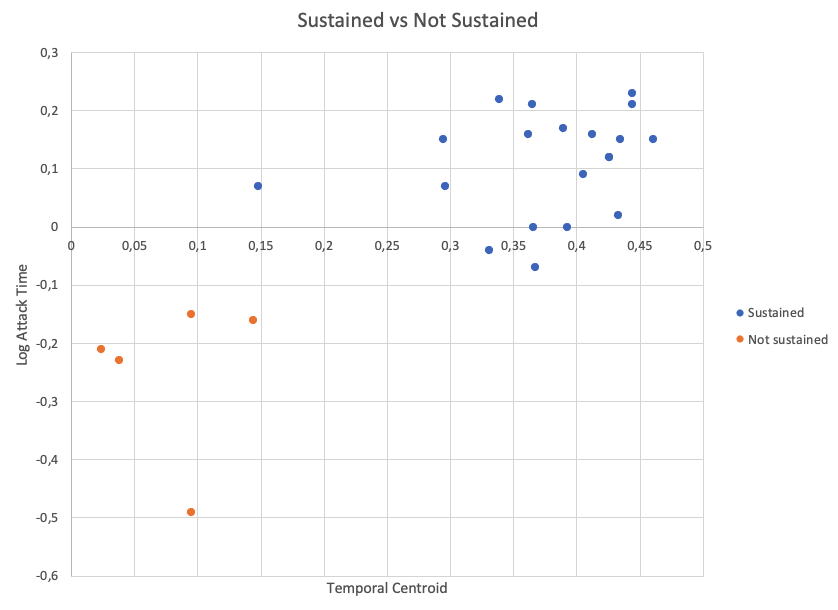
\includegraphics[width=.8\linewidth]{figs/temp_cent.png}
    \caption{Sustained vs Non Sustained}
    \label{fig:3}
\end{figure}

Como podemos observar, é feita uma clara distinção entre os instrumentos sustentados como é o caso dos sopros, e não sustentados como o caso da guitarra e harpa.
Isto deve-se ao facto de os instrumentos não sustentados terem a maior parte da energia no início da onda, que leva a um \textbf{Log Attack Time} e \textbf{Temporal Centroid} baixo.


\subsection{Altura do som}

A altura de um som é a frequência percetível quando ouvimos um som.
Um indicador da frequência da onda é o \textbf{Zero Crossing Rate}, que como explicado anteriormente, reflete o número de vezes que a onda atravessa o eixo X.
Quando maior for a frequência de uma onda, mais vezes vai atravessar esse eixo.

Por outro lado, o mesmo pode ser analisado no domínio das frequências, com o \textbf{Spectral Centroid}, que indica o centro de massa da onda no espetro.
Este indicador aponta para a zona do espeto onde em média se encontra a maior parte da energia da onda.
Esta zona é a zona da frequência fundamental.

A representação destes parâmetros pode ser observada na figura \ref{fig:4}.
"Low Pitch" representa todas as notas até G3. "High Pitch" representa G4 e G5.

\begin{figure}[H]
    \centering
    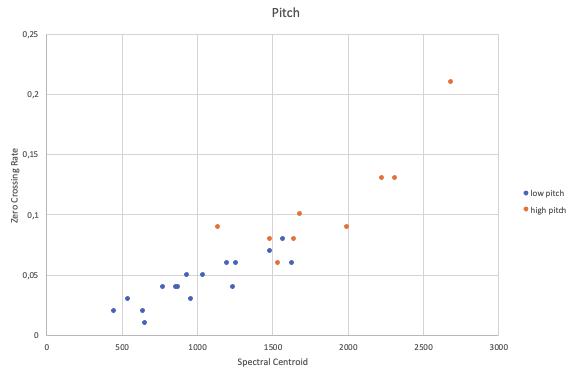
\includegraphics[width=.8\linewidth]{figs/pitch_1.png}
    \caption{Altura do Som}
    \label{fig:4}
\end{figure}

Conseguimos observar na figura \ref{fig:4} uma proporcionalidade direta entre os dois parâmetros.
Isto deve-se ao facto de ambos representarem a mesma informação, mas em domínios diferentes, pelo que este comportamento é de esperar.

A transição não é abrupta dado que de facto a maior distância que temos entre os diferentes grupos é de 1 oitava, ou 2 vezes a frequência.
No entanto, consegue observar claramente a distinção entre os diferentes sons pelo que se pode concluir que este dois parâmetros são bons indicadores para a altura do som.


\subsection{Classificação dos instrumentos de cordas}

No conjunto de samples que temos, conseguem-se identificar 5 instrumentos de cordas. O objetivo é determinar um par de parâmetros que nos permita distinguir estes instrumentos dentro da mesma família.
O primeiro parâmetro considerado foi o \textbf{Log Attack Time}. Este indicador determina o tempo que se demora a atingir 90\% da amplitude máxima.
Em instrumentos percutidos, este valor é mais pequeno dado que a força que provoca o som é instantânea no início do som.
No caso de instrumentos de cordas com arco, a excitação externa que provoca o som é constante, pelo que se vai demorar mais tempo a atingir esse pico.

O segundo parâmetro é o \textbf{Spectral Spread}, que indica o desvio médio em relação ao centro de massa.
Sons quase puros indicaram um valor mais pequeno do que ruído branco, dado que a energia é toda concentrada na frequência fundamental.

Mais uma vez , instrumentos percutidos como a guitarra terão um valor mais pequeno pois a reverberação na caixa após a excitação inicial filtra o som, eliminando frequências parasitas.
No caso do violino, onde o som depende de vários elementos não discretos como é o caso do dedo e da posição do arco, o valor deverá ser mais alto.

A representação destes parâmetros pode ser observada na figura \ref{fig:5}.

\begin{figure}[H]
    \centering
    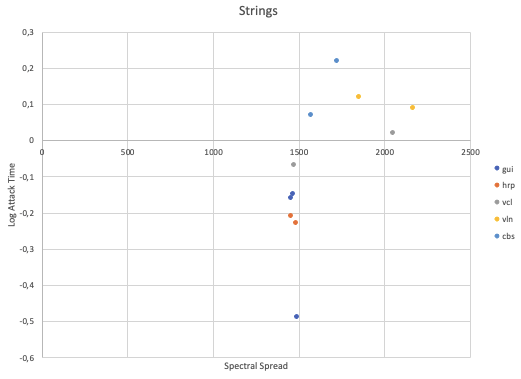
\includegraphics[width=.8\linewidth]{figs/string_1.png}
    \caption{Instrumentos de cordas}
    \label{fig:5}
\end{figure}

Como se pode observar, é feita uma clara distinção entre instrumentos percutidos como é o caso da guitarra e da harpa, de instrumentos com arco.
Dentro de cada grupo, a distinção é mais difícil. No caso dos instrumentos percutidos, o \textbf{Log Attack Time} pode ser um indicador para distinguir dado que geralmente é muito similar mesmo para diferentes frequências.

No caso dos instrumentos de arco, o \textbf{Log Attack Time} não é um bom indicador pois varia muito com a interpretação.
Aqui, o \textbf{Spectral Spread} é mais indicado pois reage às diferenças a nível de ressonância dos diferentes instrumentos.


\subsection{Classificação dos instrumentos de sopro}

Por último, procedemos à classificação dos instrumentos de sopro. Temos um total de 6 instrumentos, tanto madeiras como metais.
Neste caso, a excitação dos diferentes instrumentos é similar e a sua distinção pode ser mais difícil.
Foi escolhido o \textbf{Spectral Spread} mais um vez por ser um bom indicador das diferentes propriedades sonoras de cada instrumentos.
Com este parâmetro ja conseguimos fazer alguma distinção com instrumentos como o acordeão a terem um valor mais alto e trompa/tuba mais baixo.

O outro parâmetro escolhido foi o \textbf{Spectral Flatness}, que à semelhança do \textbf{Spectral Spread}, indica o nível de ruído do som.
Um valor próximo de 0 indica um som puro e um próximo de um ruído puro. É de notar que os valores apresentados forma multiplicados por 1000 para facilitar a sua análise.
Deste modo, apesar de estes dois parâmetros estarem altamente correlacionados, não é possível verificar isso com as amostras disponíveis.
Este parâmetro ajuda a distinguir  alguns instrumentos de forma clara como é o caso da flauta e do clarinete.

\begin{figure}[H]
    \centering
    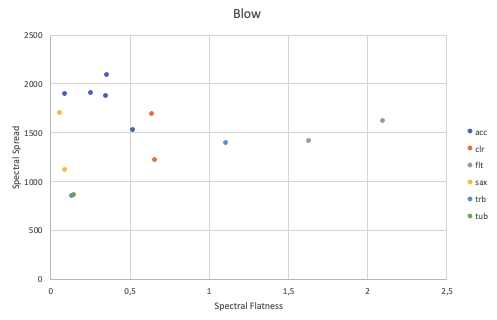
\includegraphics[width=.8\linewidth]{figs/blow_1.png}
    \caption{Instrumentos de Sopro}
    \label{fig:6}
\end{figure}

No gráfico podemos distinguir com facilidade instrumentos como o acordeão saxofone, clarinete e flauta. 
No entanto, trompa e trombone apresentam valores muito similares e uma maior amostra maior assim como mais parâmetros é necessário para retirar mais conclusões.

\section{Task 4} \label{ex_4}

Uma possível aplicação deste conhecimento a nível de aplicações multimedia é identificação musical.
Podemos utilizar estes diferentes parâmetros para identificar corretamente um música, fazendo correspondência com uma base de dados.
Dado que o processo é automatizado, é possível processar grandes quantidades de música, criando uma base de dados extensa.
É mais fácil comparar com alguns descritores que são "arrays" de dados do que o ficheiro sonoro completo, podendo dessa forms obter uma resposta em tempo real.
Um exemplo prático é o caso do \textbf{Shazam}.

\section{Task 5} \label{ex_5}

Nesta secção é feito uso da informação obtida nas secções anteriores para classificar as diferentes samples:
\begin{itemize}
    \item Sustentado / Não Sustentado
    \item Categorizarão nas cordas quanto ao instrumentos
    \item Categorizarão nos sopros quanto ao instrumentos
    \item Percussão / Não percussão não é feita pois não há samples. É feita uma análise de instrumentos percutidos e não percutidos nas cordas.
\end{itemize}

Com base no dados obtidos anteriormente, criamos um conjunto de regras para classificar os instrumentos e analisamos a sua precisão.
Estas regras foram representadas no gráfico para facilitar a sua compreensão.

\subsection{Sustentação}

\begin{figure}[H]
    \centering
    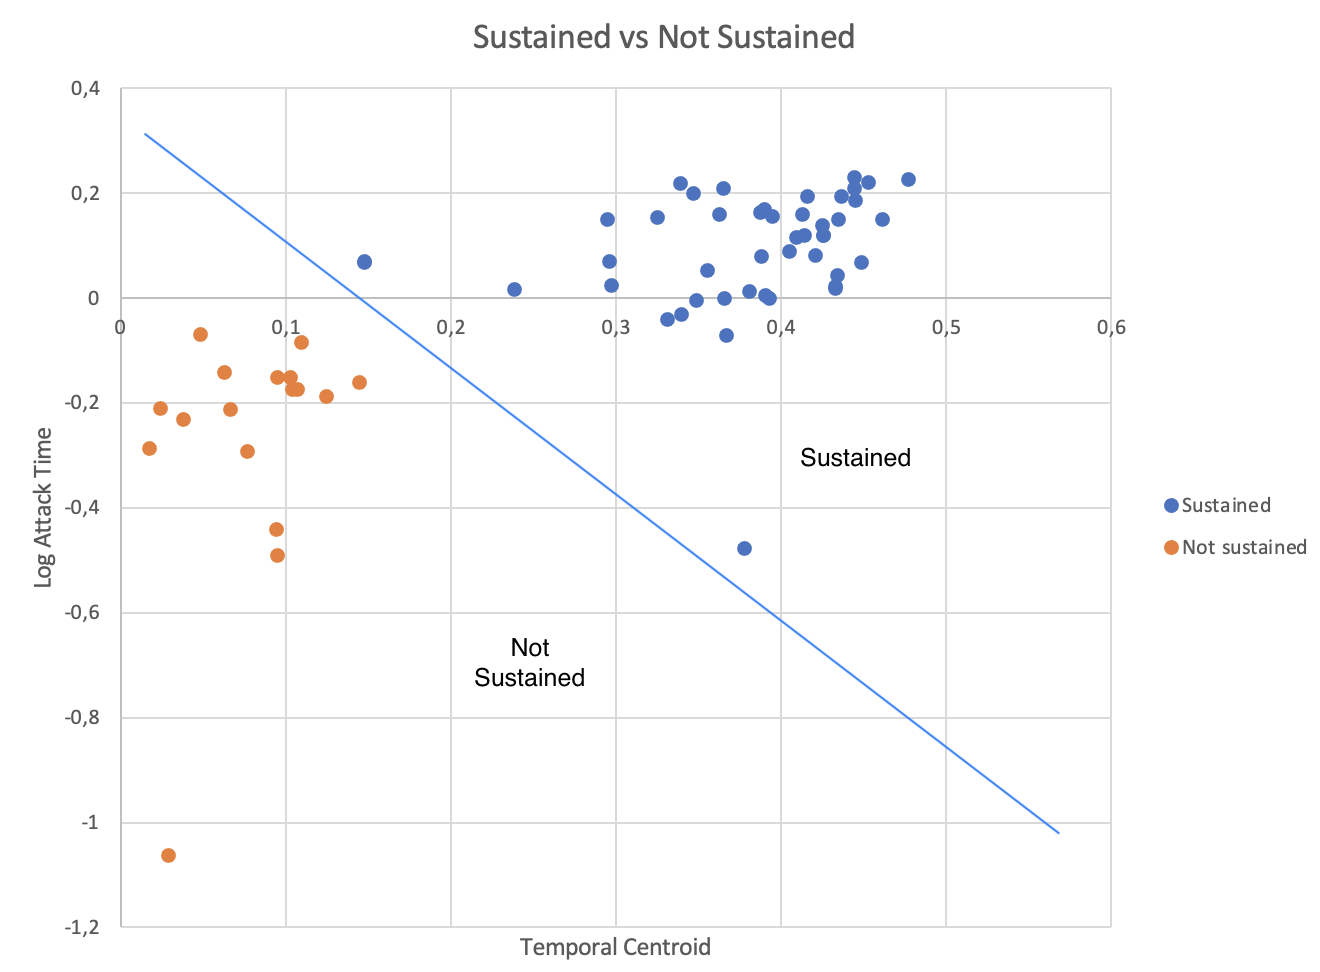
\includegraphics[width=.8\linewidth]{figs/comp_4.png}
    \caption{Instrumentos de Sopro}
    \label{fig:10}
\end{figure}

Para distinguir um som quanto à sustentação, definimos a regra como mostrado na figura \ref{fig:10}.
Um som não sustentado tem \textbf{Log Attack Time} e \textbf{Temporal Centroid} elevados e vise-versa, o que torna a divisão fácil.
Conseguimos com os dados obtidos obter um precisão de 100\%.
É preciso salvaguardar que a normalização dos Log Attack Time não foi feita de forma correta e portanto os seus valores podem não representar a realidade.
No entanto, a normalização foi feita de forma uniforme logo os valores são comparáveis.

\subsection{Cordas}

\begin{figure}[H]
    \centering
    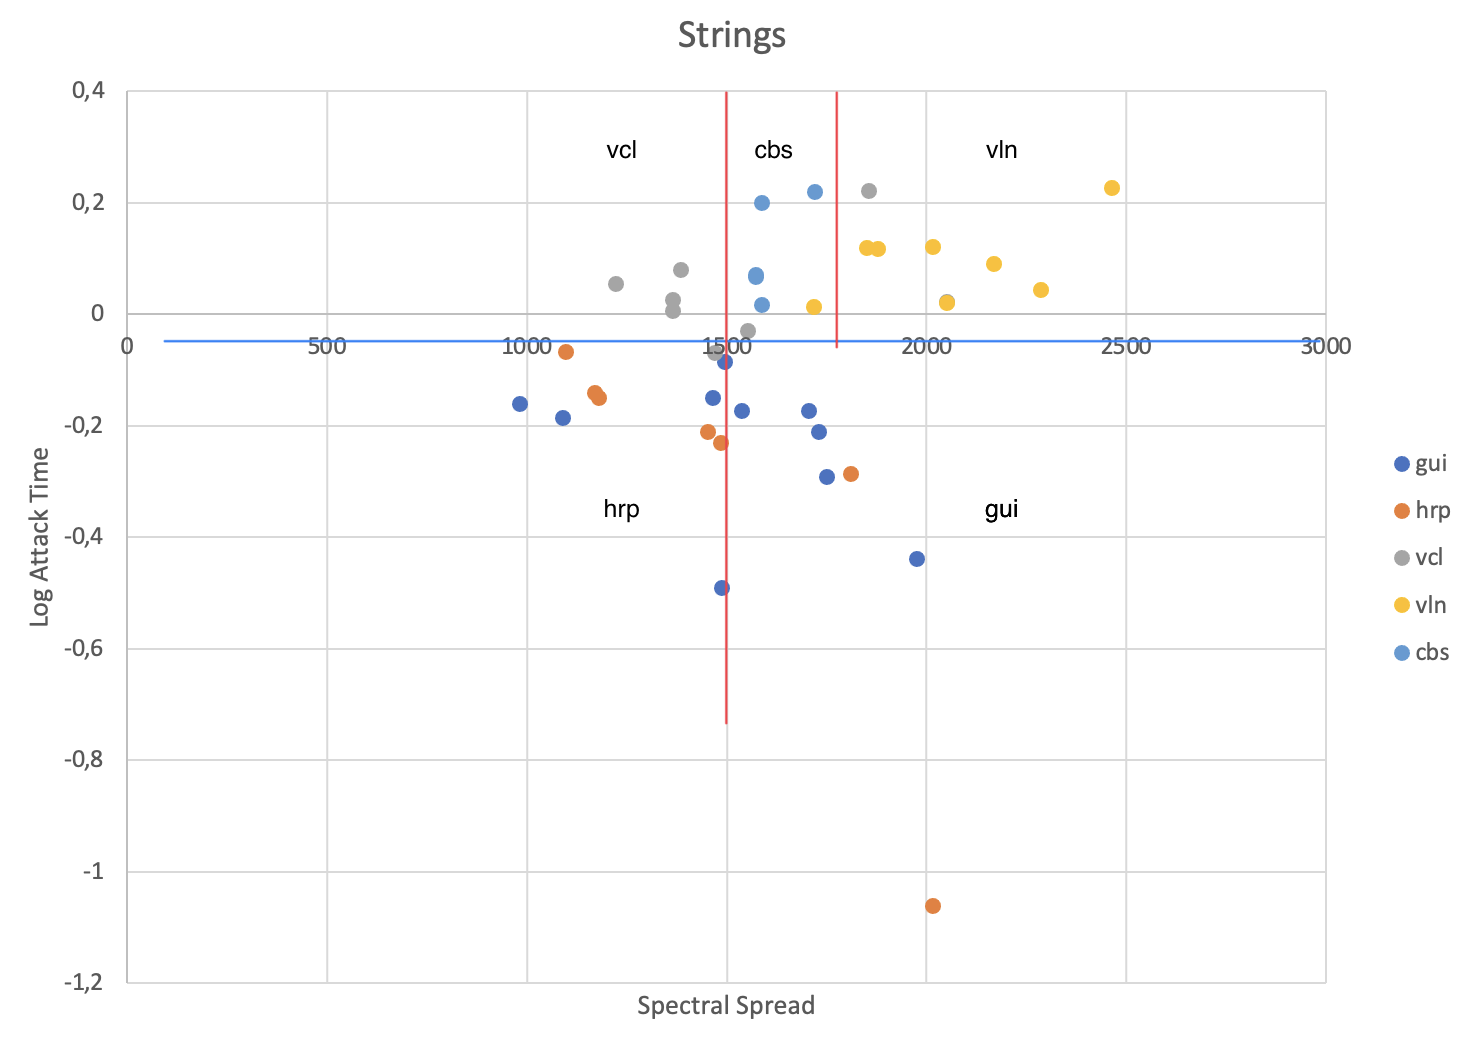
\includegraphics[width=.8\linewidth]{figs/comp_2.png}
    \caption{Instrumentos de Cordas}
    \label{fig:8}
\end{figure}

Na distinção entre os instrumentos de cordas, mais uma vez representamos no gráficos as linhas de decisão.
Os instrumentos Guitarra e harpa são difíceis de distinguir com estes parâmetros.
As suas características são parecidas e seriam precisos outros parâmetros para os identificar.
As samples da harpa em específico apresentam valores pouco constantes, o que torna difícil a sua categorizarão.
A modificação dos parâmetros das funções como o tamanho da janela pode obter valores mais constantes.
Obtemos 28 corretos, 10 incorretos, com uma precisão de $\frac{28}{38} \approx 73.7\%$.


\subsection{Percutidos}

\begin{figure}[H]
    \centering
    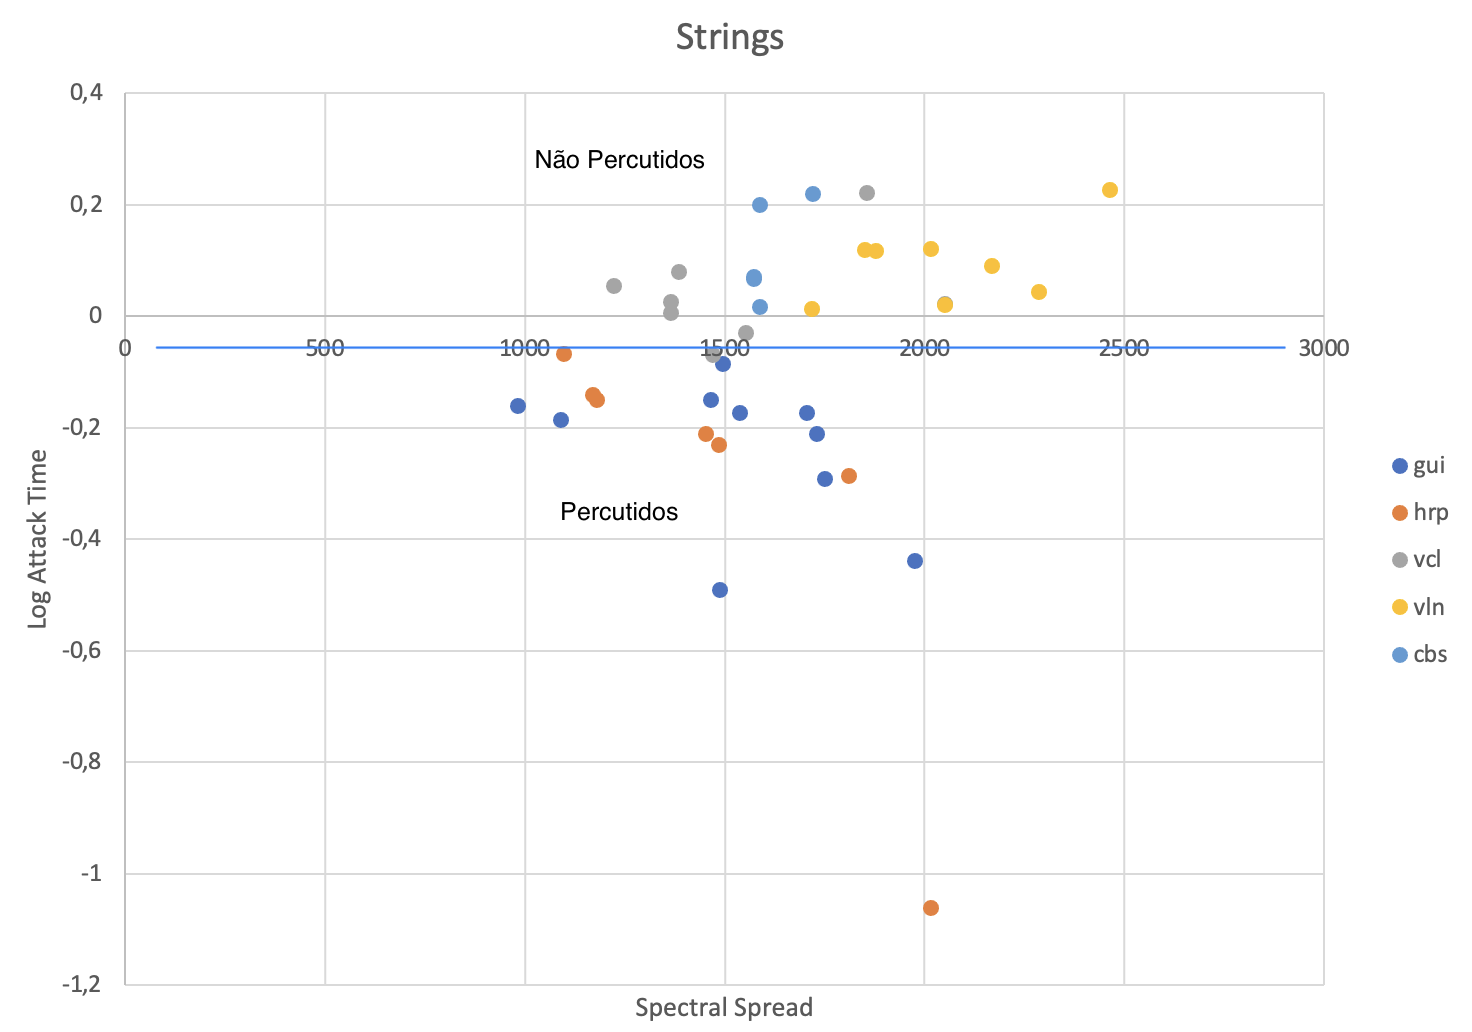
\includegraphics[width=.8\linewidth]{figs/comp_1.png}
    \caption{Percutidos / Não Percutidos}
    \label{fig:7}
\end{figure}

Como explicado anteriormente, instrumentos percutidos geralmente têm um log attack time mais baixo. 
O Spectral Spread não é relevante nesta classificação mas é importante para distinguir os instrumentos entre si.
Obtemos então 37 corretos, 1 incorreto, com uma precisão de $\frac{37}{38} \approx 97.4\%$.


\subsection{Sopro}

\begin{figure}[H]
    \centering
    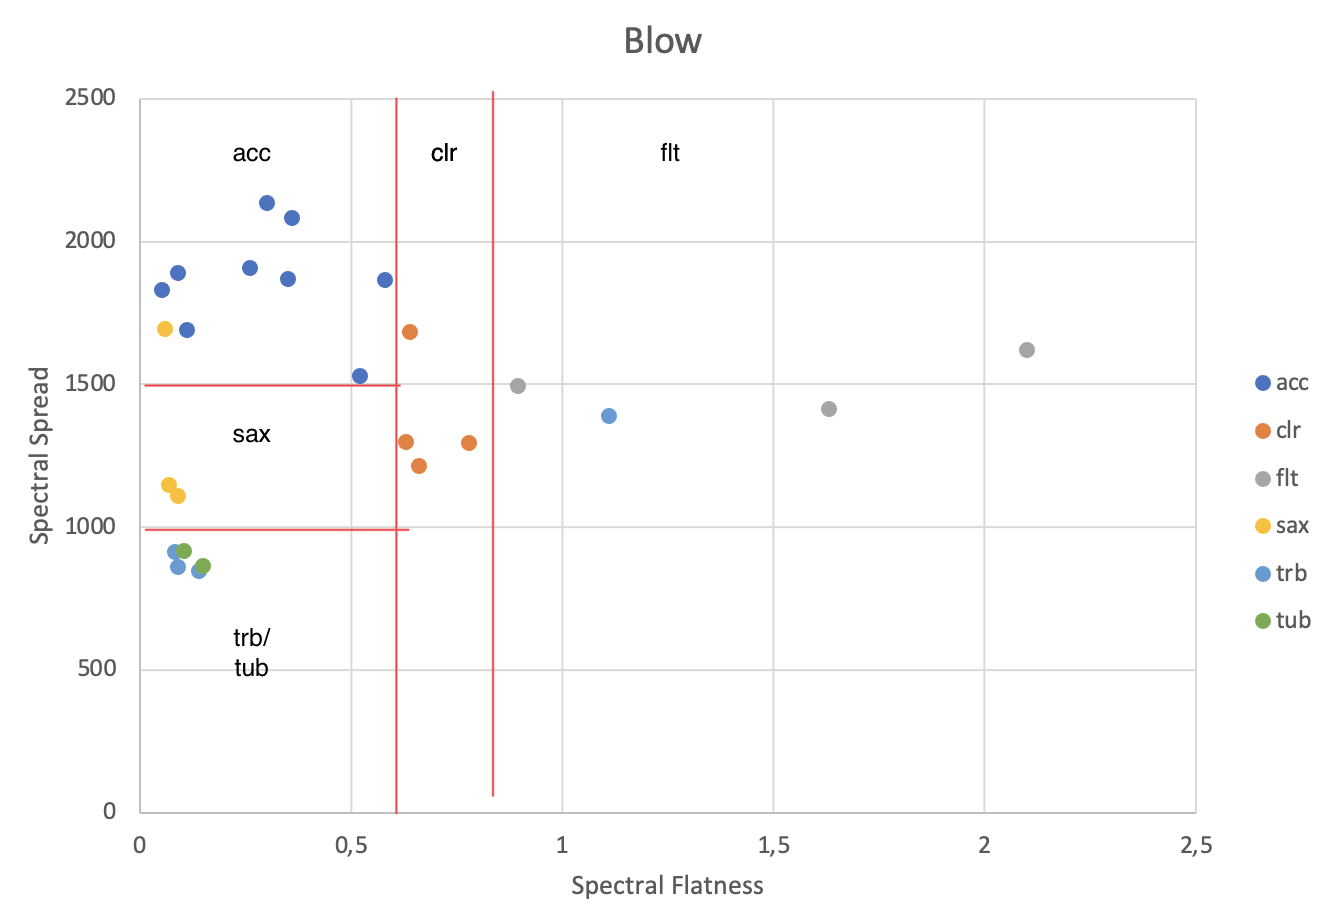
\includegraphics[width=.8\linewidth]{figs/comp_3.png}
    \caption{Instrumentos de Sopro}
    \label{fig:9}
\end{figure}

De uma forma geral conseguimos distinguir bem os instrumentos. 
A exceção é no caso da trompa e tuba, que apresentam parâmetros idênticos.
De uma forma similar à guitarra e harpa, a trompa e a tuba são instrumentos similares e distinguem-se principalmente pelo registo que tocam.
Seriam então necessários outros parâmetros para distinguir, sendo que neste caso consideramos um classificação conjunta.
Obtemos 23 corretos, 2 incorretos, com uma precisão de $\frac{23}{25} = 92\%$.






